% $Header: /Users/joseph/Documents/LaTeX/beamer/solutions/conference-talks/conference-ornate-20min.en.tex,v 90e850259b8b 2007/01/28 20:48:30 tantau $

\documentclass{beamer}

% This file is a solution template for:

% - Talk at a conference/colloquium.
% - Talk length is about 20min.
% - Style is ornate.



% Copyright 2004 by Till Tantau <tantau@users.sourceforge.net>.
%
% In principle, this file can be redistributed and/or modified under
% the terms of the GNU Public License, version 2.
%
% However, this file is supposed to be a template to be modified
% for your own needs. For this reason, if you use this file as a
% template and not specifically distribute it as part of a another
% package/program, I grant the extra permission to freely copy and
% modify this file as you see fit and even to delete this copyright
% notice. 


\mode<presentation>
{
  \usetheme{Warsaw}
  % or ...

  \setbeamercovered{transparent}
  % or whatever (possibly just delete it)
  %\useoutertheme[footline=authortitle]{miniframes}
}

\setbeamercolor{note}{fg=black,bg=lightgray} 
\usepackage[english]{babel}
% or whatever

\usepackage[latin1]{inputenc}
% or whatever

\usepackage{times}
\usepackage[T1]{fontenc}
% Or whatever. Note that the encoding and the font should match. If T1
% does not look nice, try deleting the line with the fontenc.


\title[Partitioning students into equitable groups] % (optional, use only with long paper titles)
{Partitioning of students into equitable groups using SolverStudio}

% \subtitle
% {Include Only If Paper Has a Subtitle}

\author[Michael Fairley and Oscar Dowson] % (optional, use only with lots of authors)
{Michael Fairley \and Oscar Dowson}
% - Give the names in the same order as the appear in the paper.
% - Use the \inst{?} command only if the authors have different
%   affiliation.

\institute[University of Auckland] % (optional, but mostly needed)
{
  Department of Engineering Science\\
  University of Auckland
}
% - Use the \inst command only if there are several affiliations.
% - Keep it simple, no one is interested in your street address.

\date[] % (optional, should be abbreviation of conference name)
{2014 Joint NZSA+ORSNZ Conference}
% - Either use conference name or its abbreviation.
% - Not really informative to the audience, more for people (including
%   yourself) who are reading the slides online

\subject{Operations Research}
% This is only inserted into the PDF information catalog. Can be left
% out. 



% If you have a file called "university-logo-filename.xxx", where xxx
% is a graphic format that can be processed by latex or pdflatex,
% resp., then you can add a logo as follows:

% \pgfdeclareimage[height=0.5cm]{university-logo}{university_logo.eps}
% \logo{\pgfuseimage{university-logo}}



% Delete this, if you do not want the table of contents to pop up at
% the beginning of each subsection:
% \AtBeginSubsection[]
% {
%   \begin{frame}<beamer>{Outline}
%     \tableofcontents[currentsection,currentsubsection]
%   \end{frame}
% }


% If you wish to uncover everything in a step-wise fashion, uncomment
% the following command: 

%\beamerdefaultoverlayspecification{<+->}


\begin{document}

\begin{frame}
  \titlepage
\end{frame}

\begin{frame}{Outline}
  \tableofcontents
  % You might wish to add the option [pausesections]
\end{frame}


% Structuring a talk is a difficult task and the following structure
% may not be suitable. Here are some rules that apply for this
% solution: 

% - Exactly two or three sections (other than the summary).
% - At *most* three subsections per section.
% - Talk about 30s to 2min per frame. So there should be between about
%   15 and 30 frames, all told.

% - A conference audience is likely to know very little of what you
%   are going to talk about. So *simplify*!
% - In a 20min talk, getting the main ideas across is hard
%   enough. Leave out details, even if it means being less precise than
%   you think necessary.
% - If you omit details that are vital to the proof/implementation,
%   just say so once. Everybody will be happy with that.

\section{Motivation}

\subsection{ENGGEN 403: Managing a Business}

\begin{frame}{The systems engineering group project}
  \begin{itemize}
    \item All final year engineering students
    \item \textasciitilde600 students divided into groups of 25
    \item One week
  \end{itemize}
\end{frame}

\begin{frame}{What is an equitable group?}


\end{frame}

\subsection{Previous Method}
\begin{frame}{Previous Method}
  \begin{itemize}
    \item Manual
    \item Akin to sequential greedy algorithm
    \item Time consuming (\textasciitilde 2 days)
    \item Difficult to train future course organisers
  \end{itemize}
\end{frame}

\section{Our Solution}

\subsection{Model}
\begin{frame}{Mixed Integer Programme}
\begin{itemize}
  \item Decision variables
  \begin{itemize}
    \item binary, assign each student to a group
  \end{itemize}
  \pause
  \item Objective function
  \begin{itemize}
    \item minimise spread of group mean GPA
    \item minimise spread of group GPA variance
  \end{itemize}
  \pause
  \item Constraints
  \begin{itemize}
    \item evenly distribute gender, discipline, ethnicity
    \item calculate group mean GPA and variance
  \end{itemize}
  \pause
  \item Data
    \begin{itemize}
     \item university held student records
    \end{itemize}
\end{itemize}
\end{frame}
\subsection{Implementation}
\begin{frame}{Microsoft Excel Spreadsheet}
\begin{itemize}
  \item SolverStudio plug-in
  \item PuLP modelling language
  \item COIN-OR CBC solver
  \item End user only needs existing Excel skills
\end{itemize}
\end{frame}
\begin{frame}{Interface Screenshot}
\centering
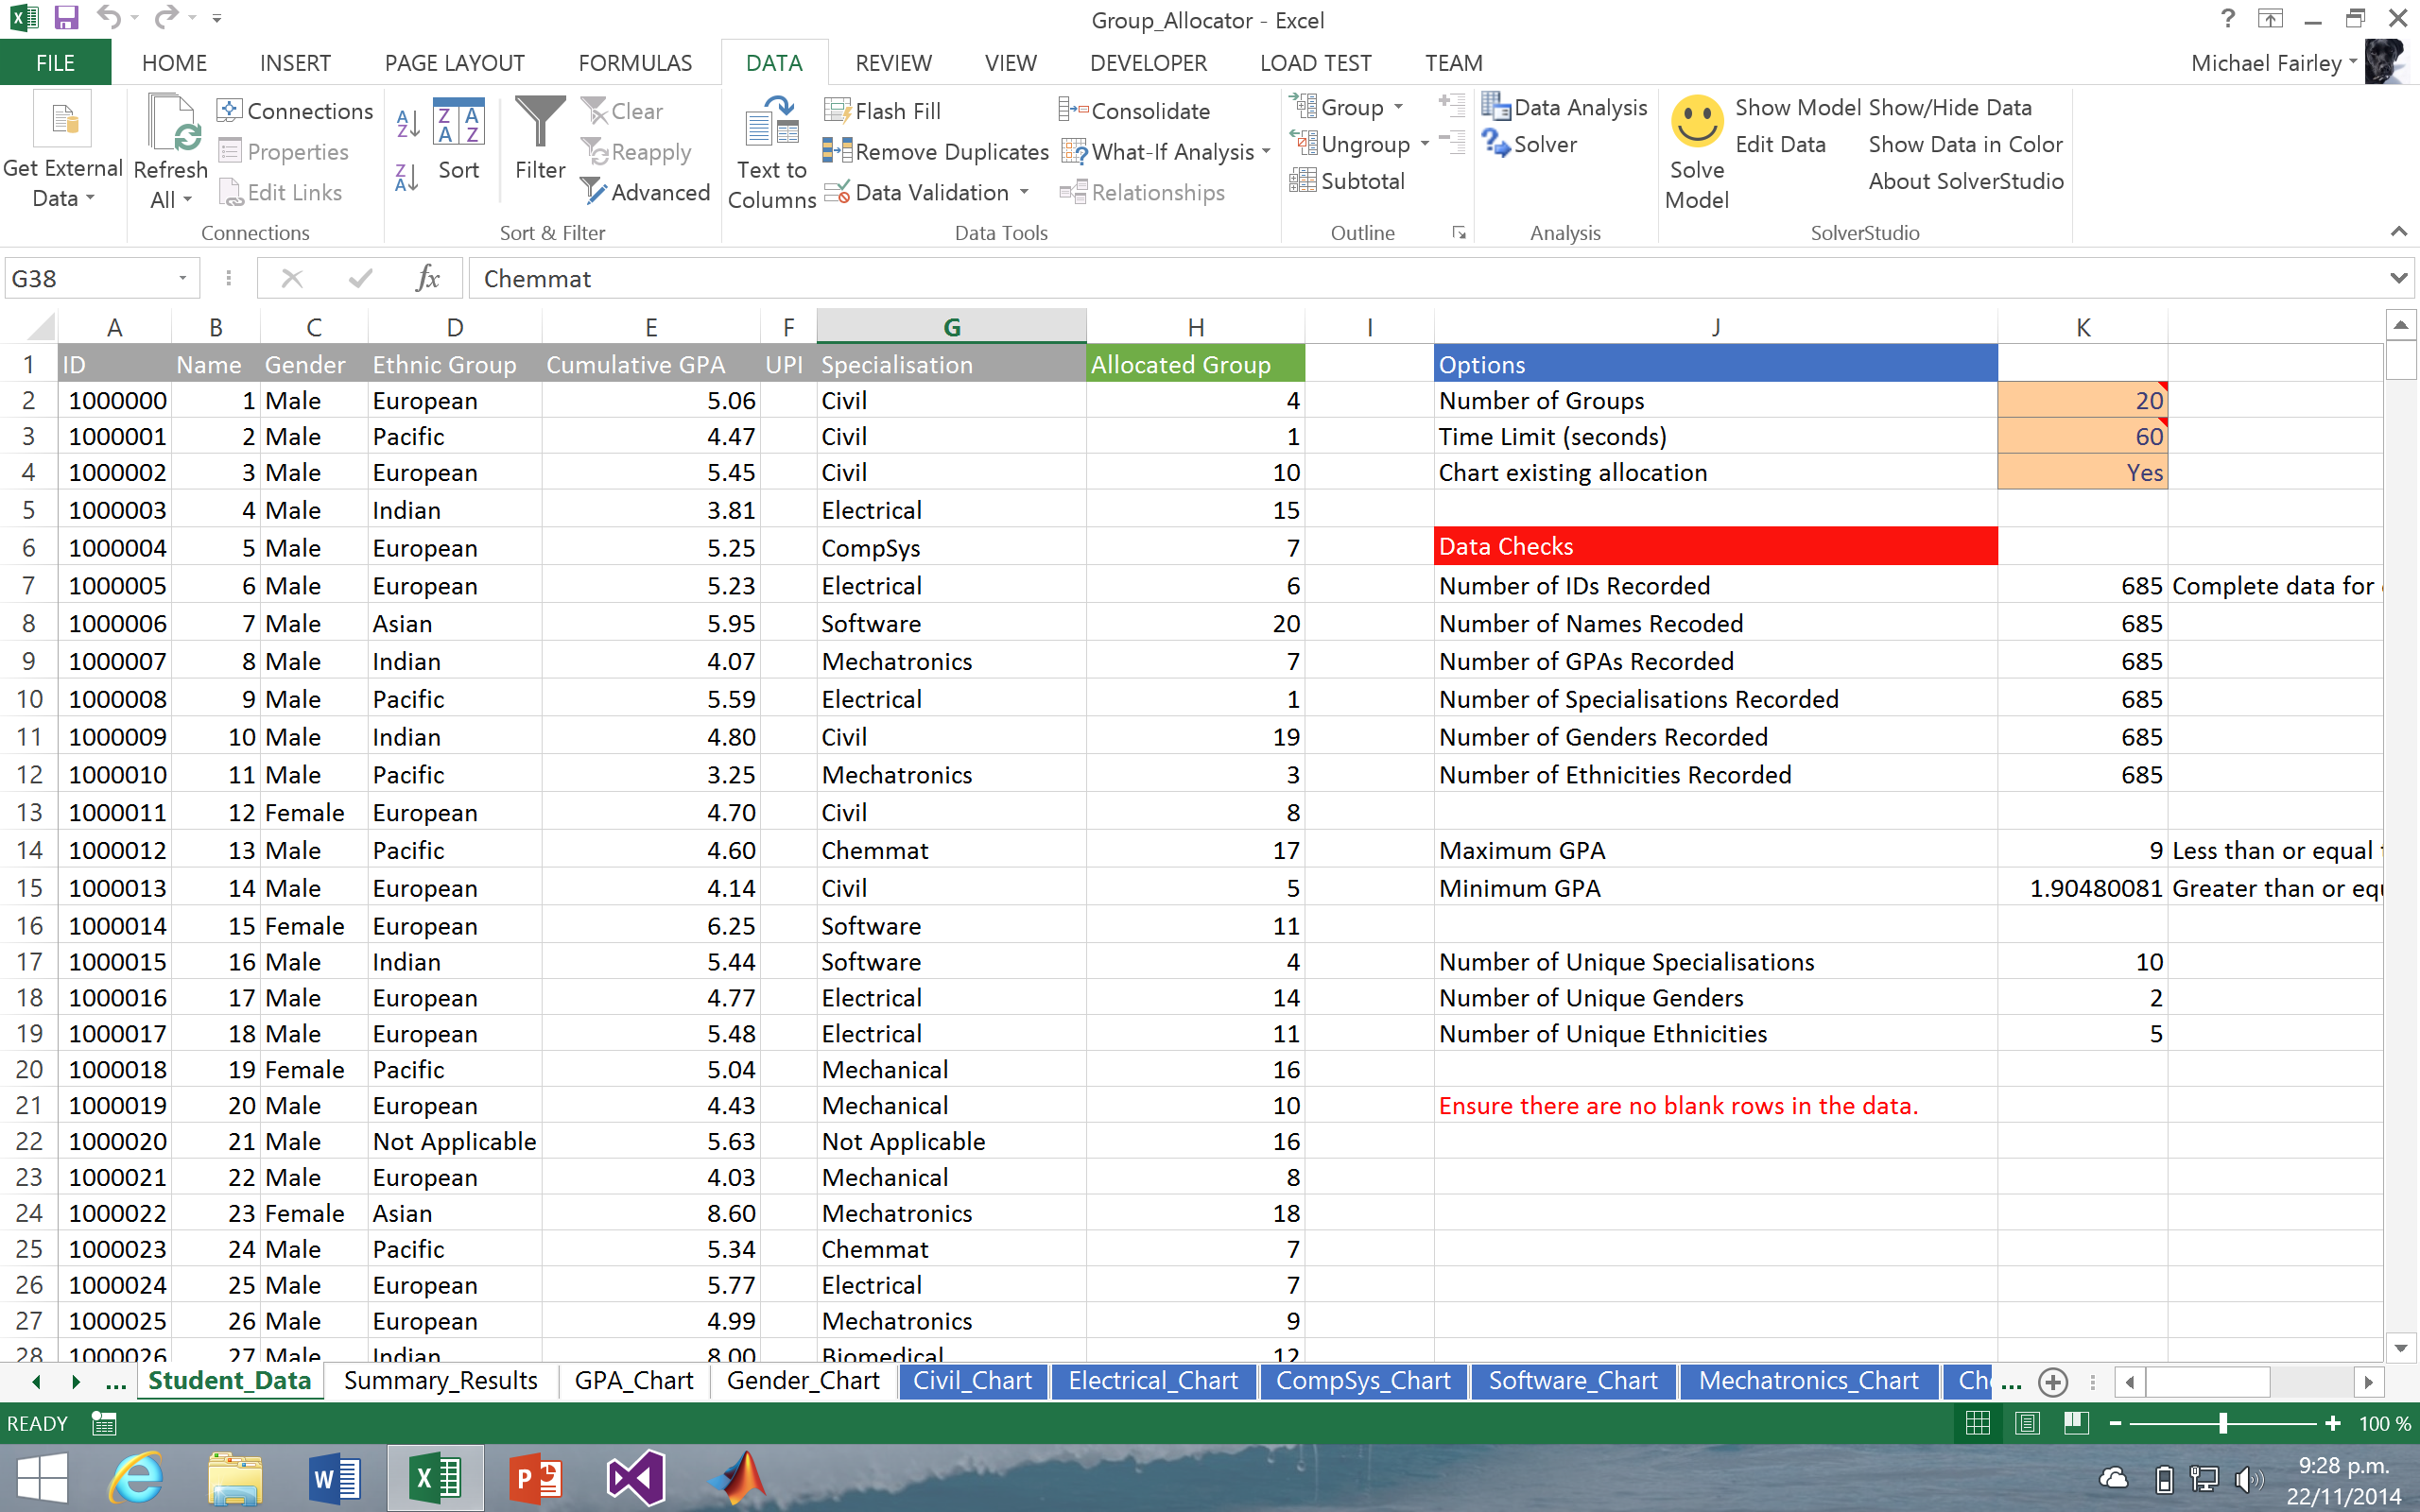
\includegraphics[width=11cm]{screenshot.png}
\end{frame}
\begin{frame}{Visualisation Tools}
\centering
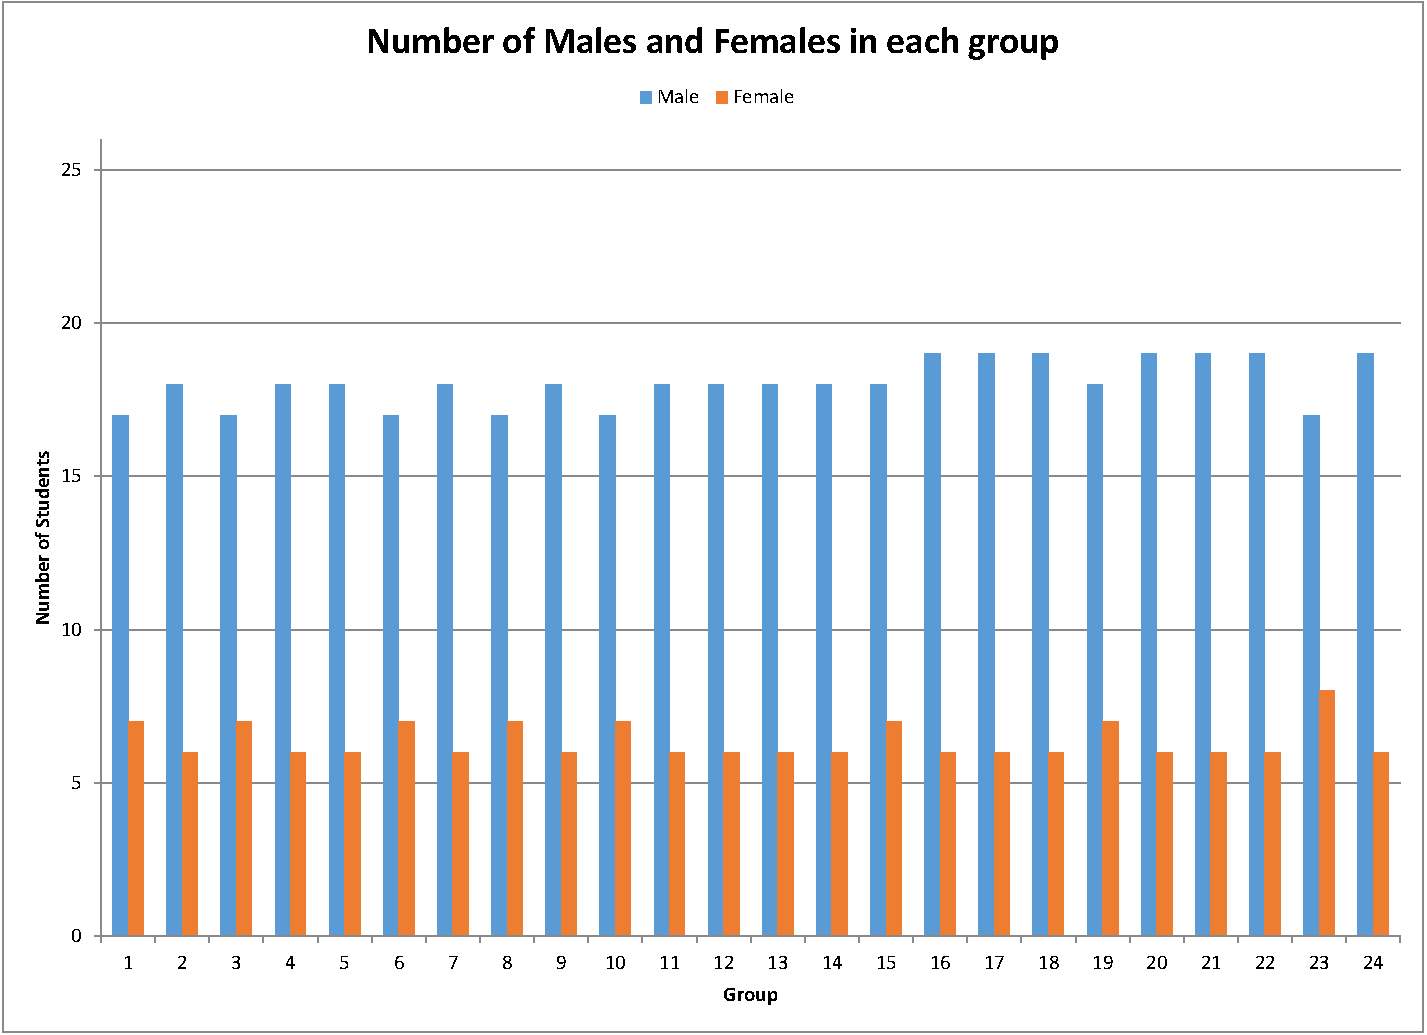
\includegraphics[height=3.8cm]{bar_chart.pdf}
\hfill
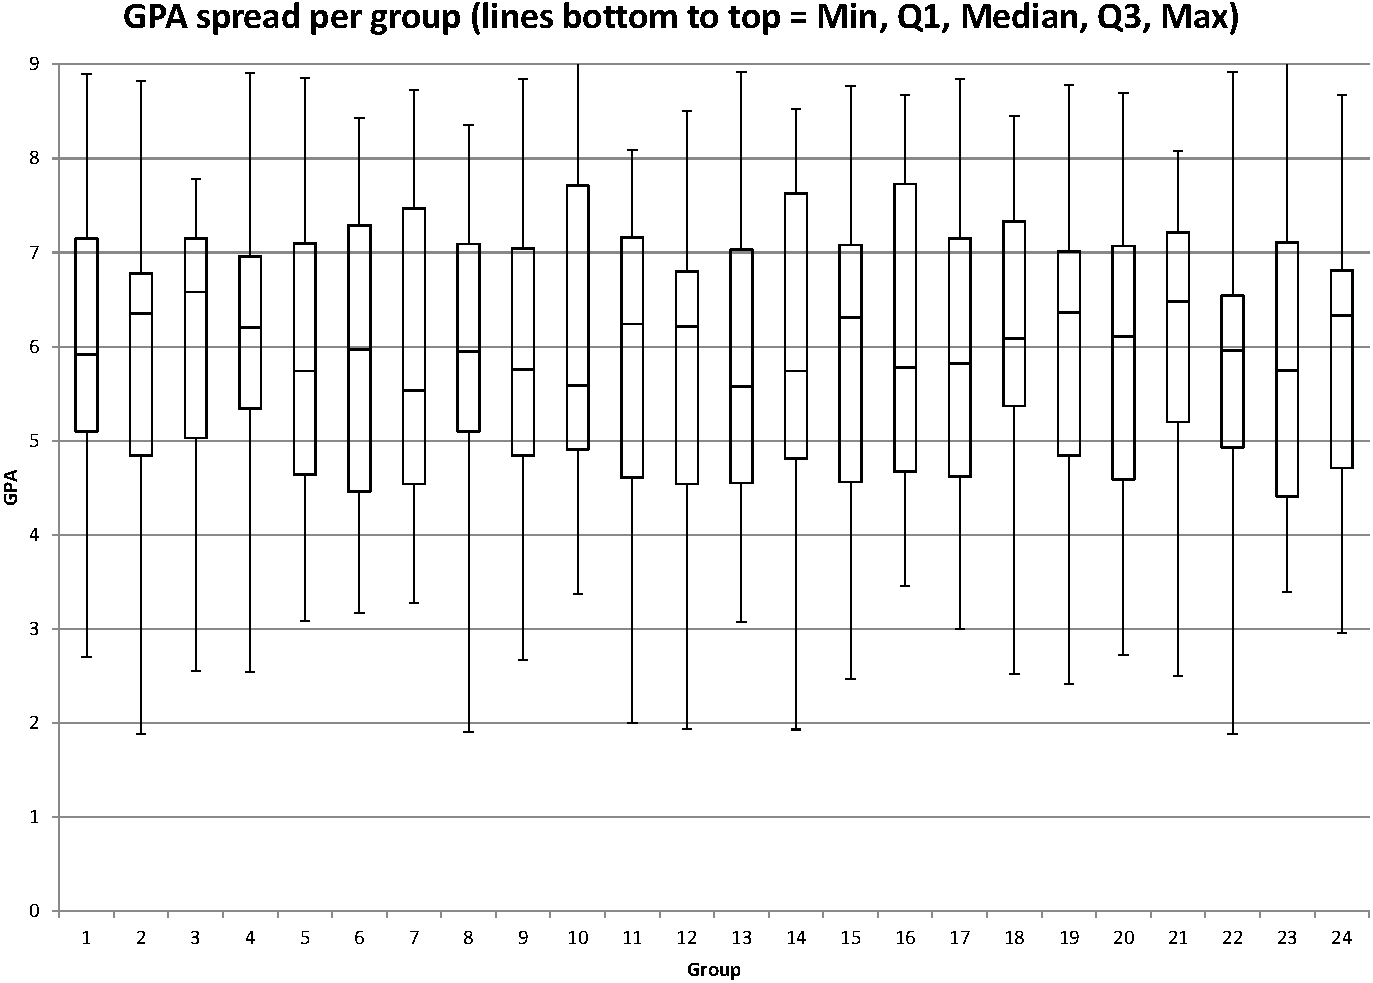
\includegraphics[height=3.8cm]{gpa.pdf}
\begin{itemize}
\item Automatically generated charts
\end{itemize}
\end{frame}
\subsection{Validation}
\begin{frame}{Solution compared with 2013 manual allocation}
  \begin{itemize}
    \item Manual allocation in 2013 provided benchmark
    \item Optimisation mostly better than manual
    \item Difficult to compare solutions
    \item Optimisation much faster (2 min vs 2 days)
  \end{itemize}
\end{frame}
\begin{frame}{Optimisation markedly reduced GPA spread}
\centering
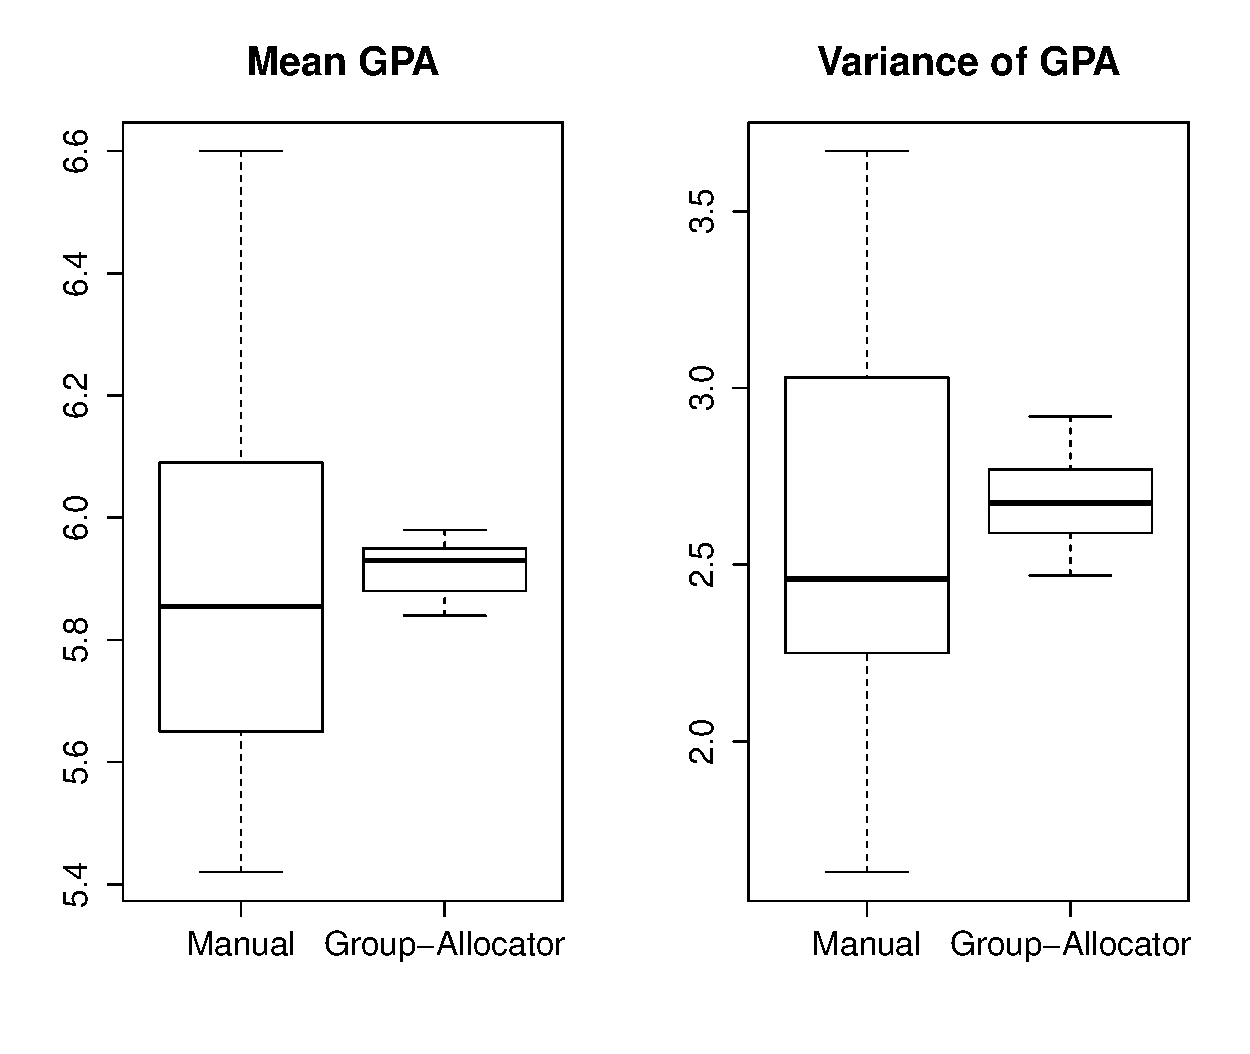
\includegraphics[height=6cm]{gpa_plot.pdf}
\end{frame}

\section*{Summary}
\begin{frame}{Summary}
\begin{itemize}
  \item Model formulated to allocate students to groups
  \item Combination of Excel, SolverStudio and PuLP lead to quick implementation time and easy to use interface for end user
  \item From idea to real-world application only took 2 weeks
  \item Groups successfully allocated in 2014
\end{itemize}
\end{frame}

{
 \usebackgroundtemplate{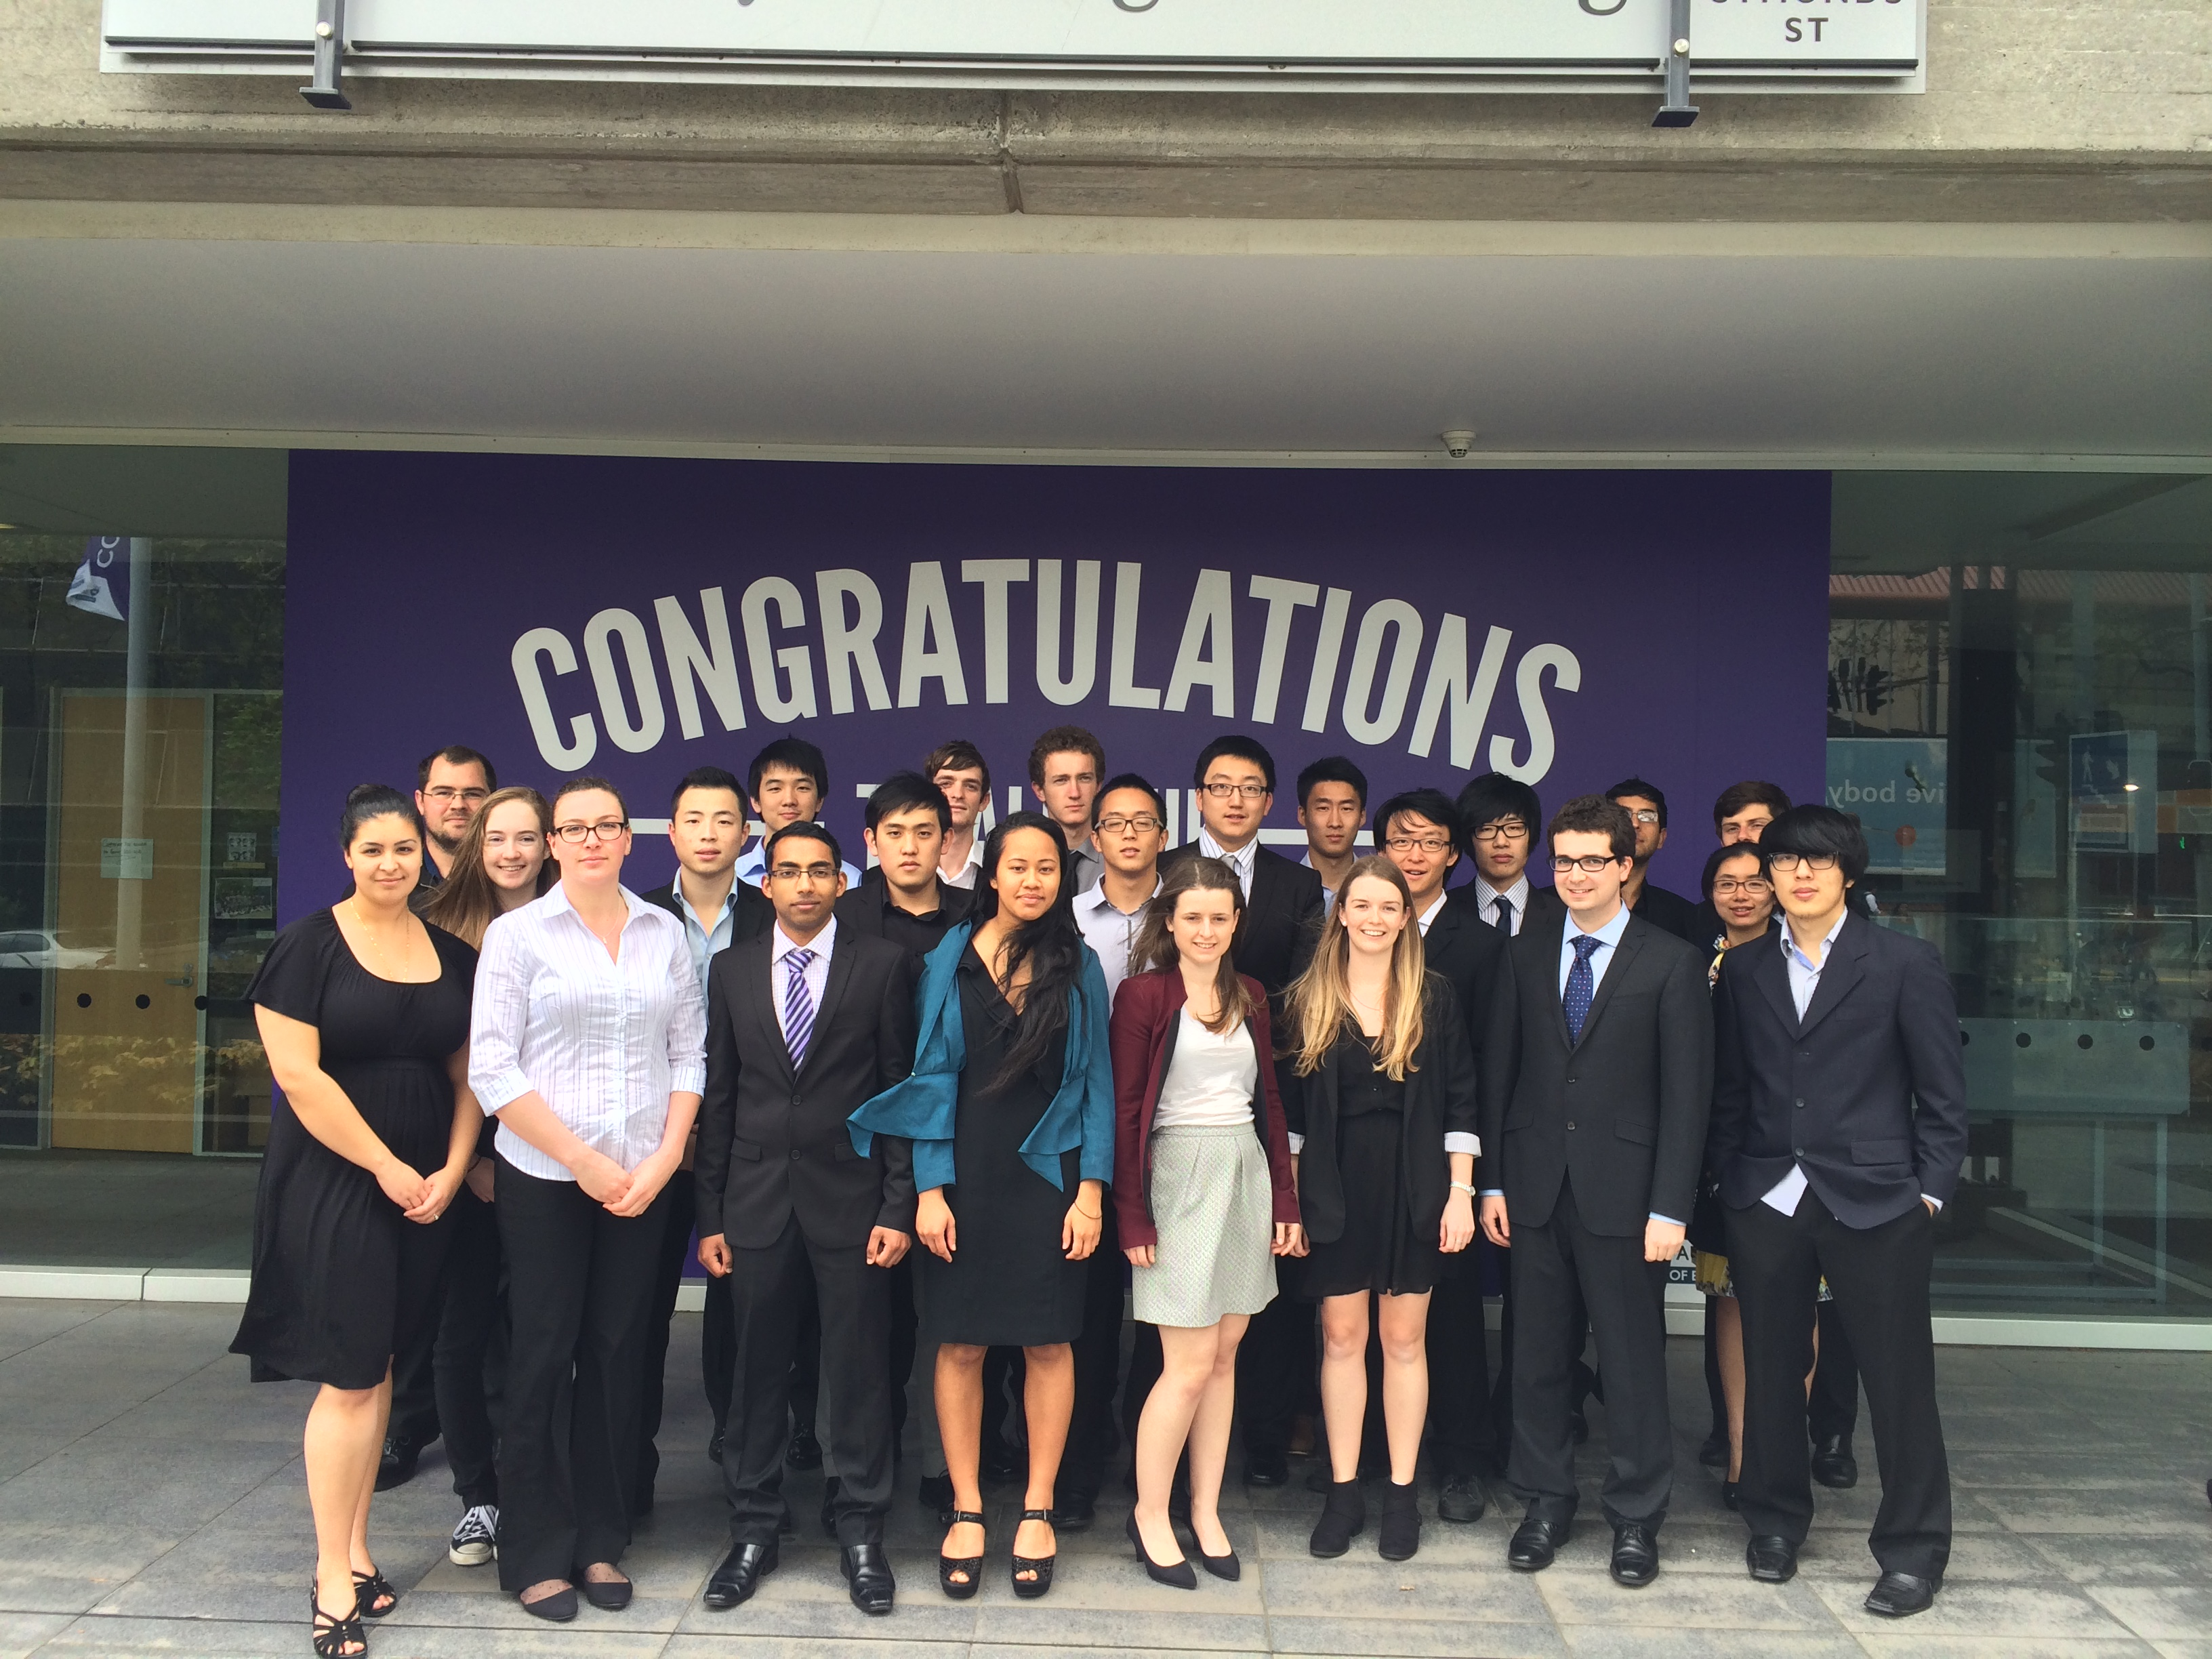
\includegraphics[width=\paperwidth]{group.JPG}} 

 \begin{frame}[plain]

 \end{frame}
}

\begin{frame} 
\begin{beamercolorbox}[center,shadow=true,rounded=true,]{note} 
        Questions? 
\end{beamercolorbox}

% \begin{block}{Spreadsheet download link}
% http://github.com/odow/group-allocator
% \end{block}

\end{frame} 

\end{document}


